% arara: xelatex: {synctex: true}
% arara: indent: {overwrite: yes}
\documentclass[]{IMTexam}

\usepackage{IMTtikz}

\givecredits
\author{Isabella B.}
\USPN{11810773}
\date{}
\lecture{Física I} % disciplina
\lcode{4302111}
\hwtype{Resolução} % o que é
\examname{Lista 7} % prova

\begin{document}

\maketitle

\begin{questions}

	\question Considere um triângulo equilátero, da lado $ L $ e densidade superficial de massa $ \sigma = \sigma_0 $ constante. Calcule a posição do centro de massa.

	\begin{solution}

	\end{solution}

	\medskip

	\question Considere uma barra de comprimento L, com densidade linear de massa dada por $ \lambda (x) = xf $, com $ f $ constante de dimensões adequadas.

	\begin{parts}
		\part Quais as dimensões físicas de $ f $?

		\begin{solution}

		\end{solution}

		\part Qual a posição do centro de massa da barra?

		\begin{solution}

		\end{solution}

		\part \label{part:q1c} Suponha que a barra seja lançada da superfície da Terra na direção vertical. Desprezando o atrito do ar, descreva a equação do movimento do centro de massa e escreva a solução supondo que a	velocidade inicial seja $ v(t = 0) = v_0 $.

		\begin{solution}

		\end{solution}

		\part Nas mesmas condições do item \ref{part:q1c}, suponha que no momento do lançamento a barra seja colocada em rotação. O que muda na trajetória do centro de massa?

		\begin{solution}

		\end{solution}
	\end{parts}

	\medskip

	\question Considere o sistema Sol-Lua-Terra, em movimento sob a ação das forças gravitacionais mútuas. Como vocês verão mais para a frente, no caso de um sistema de dois corpos que interage gravitacionalmente, a trajetória de cada um dos corpos é elíptica. Ao contrário, não existe uma solução geral analítica para um sistema de três corpos que interage gravitacionalmente. Apesar disso, o movimento do sistema Sol-Lua-Terra que está sendo considerado pode ser analisado em termos relativamente simples da forma seguinte:

	\begin{parts}
		\part Considerando que $ M_{\text{Sol}} \ll M_{\text{Terra}} \ll M_{\text{Lua}} $, mostre que é uma boa aproximação identificar o centro de massa do sistema com o centro do Sol. Qual o erro cometido nesta identificação?

		\begin{solution}

		\end{solution}

		\part Considerando que as forças externas que agem no sistema são desprezíveis, qual a trajetória do Sol no espaço?

		\begin{solution}

		\end{solution}

		\part Considerando agora que a distância média entre Terra e Sol é da ordem de \SI{1e11}{\meter}, enquanto a distância média entre Terra e Lua é de \SI{1e8}{\meter}, calcule a equação do movimento do centro de massa Terra-Lua no referencial do Sol (é um referencial inercial?), e mostre que o problema é reconduzido àquele de um sistema de dois corpos;

		\begin{solution}

		\end{solution}

		\begin{figure}
			\centering
			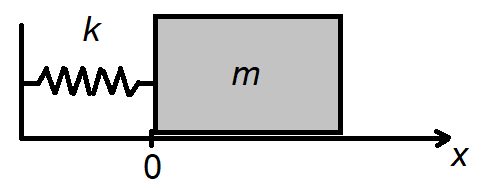
\includegraphics[width=0.7\linewidth]{screenshot001}
			\caption{Trem de comprimento L.}
			\label{fig:fig1}
		\end{figure}

		\part Em termos de quais movimentos é portanto possível descrever o sistema?

		\begin{solution}

		\end{solution}
	\end{parts}

	\medskip

	\question Calcule a expressão para a energia cinética de um sistema de $ N $ corpos no referencial do centro de massa.

	\begin{solution}

	\end{solution}

	\medskip

	\question Considere um trem de comprimento $ L $, massa total $ M $ e densidade uniforme, em movimento com velocidade $ v_0 $ num plano horizontal sem atrito (veja a figura \ref{fig:fig1}). No instante $ t = 0 $, o trem encontra uma subida retilínea que faz um ângulo $ \theta $ em relação ao plano horizontal e começa subir até parar.

	\begin{parts}
		\part Mostre explicitamente que, no cálculo da energia potencial de um corpo não puntiforme, é possível considerar um corpo puntiforme de massa igual à massa total do corpo;

		\begin{solution}

		\end{solution}

		\part \label{part:q5b} Quais as três posições possíveis nas quais o trem pode parar?

		\begin{solution}

		\end{solution}

		\part Calcule a posição do centro de massa do trem quando o trem estiver parado nas três situações do item \ref{part:q5b};

		\begin{solution}

		\end{solution}

		\part Considere agora o caso $ L = \SI{180}{\meter}, M = \SI{200x103}{\kilo\gram}, \theta  = \ang{2} $ e $ v_0 = \SI{180}{\kilo\meter\per\hour} $. Qual a altura final do centro de massa do sistema?

		\begin{solution}

		\end{solution}

		\part Escreva as equações do movimento do trem nas várias fases da subida.

		\begin{solution}

		\end{solution}
	\end{parts}

	\medskip

	\question Considere um foguete que se movimenta na vertical \textit{sob a ação de um campo gravitacional}. Qual a velocidade final do foguete após ter queimado uma parte do combustível? é melhor queimar o combustível rapidamente ou devagar?

	\begin{solution}

	\end{solution}

	\medskip

	\question Um foguete com $ N $ estágios tenta alcançar a velocidade de escape da Terra.

	\begin{figure}
		\centering
		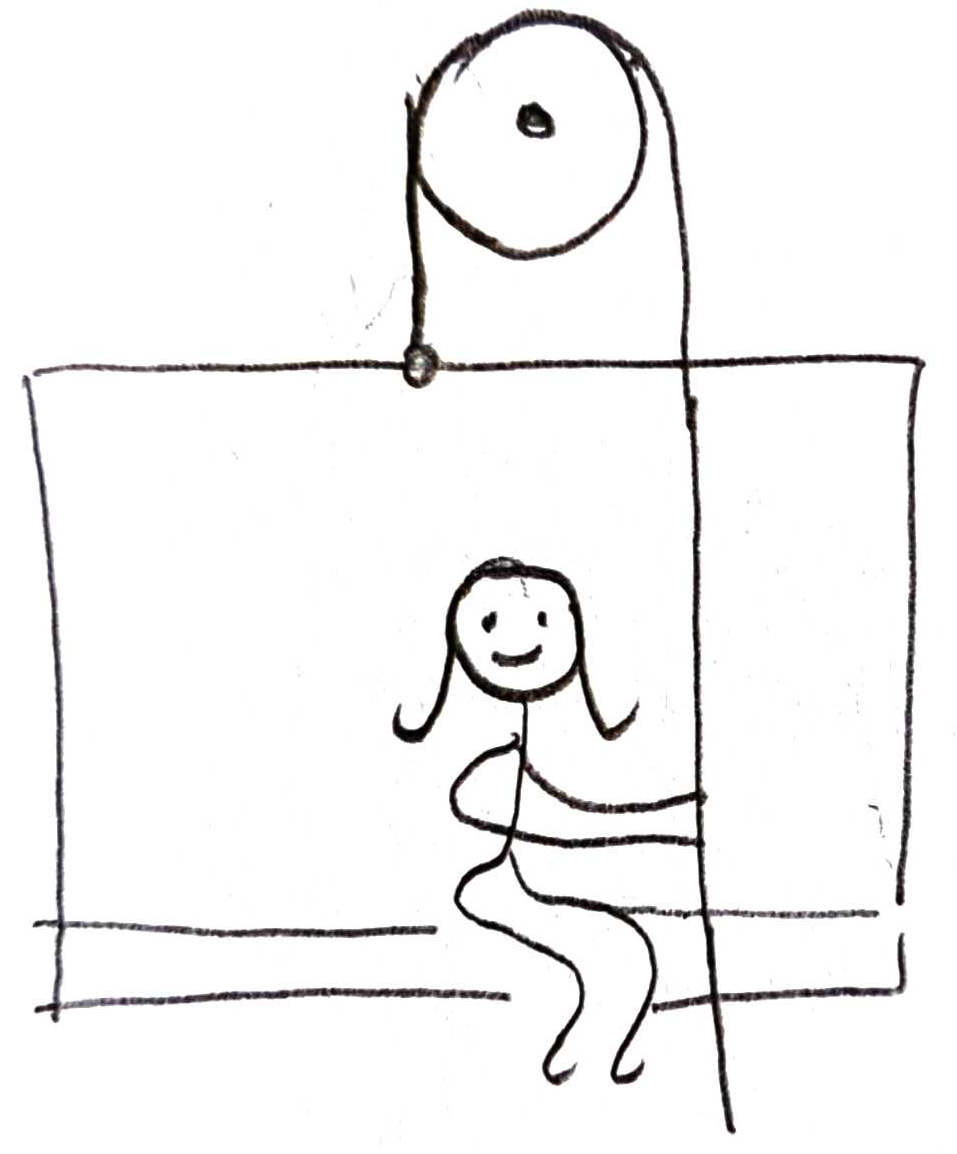
\includegraphics[width=0.7\linewidth]{screenshot002}
		\caption{International Space Station.}
		\label{fig:fig2}
	\end{figure}

	\begin{parts}
		\part Suponha que a razão entre a massa de combustível e a massa de cada um dos tanques seja de 10\%, e que a massa útil represente 1\% da massa total. Qual a velocidade final de um foguete com 3 estágios? E de um foguete com 5 estágios?

		\begin{solution}

		\end{solution}

		\part Para obter velocidades finais maiores \textit{a parte o número de estágios}, é mais eficiente diminuir a massa da carga útil em relação à massa total ou é melhor modificar a razão entre a massa do combustível e a massa dos tanques?

		\begin{solution}

		\end{solution}
	\end{parts}

	\medskip

	\question Num satélite em órbita baixa ao redor da Terra atua uma força de atrito devida à atmosfera do planeta. Essa força de atrito se opõe ao movimento, causando uma diminuição do raio da órbita do satélite. Por exemplo, a Figura \ref{fig:fig2} mostra a altura da \textit{International Space Station} (ISS) em função do tempo, onde podemos claramente identificar os períodos de queda e os períodos (rápidos) onde uma parte do combustível é usada para aumentar a altura. Dado que o atrito é fraco, em cada instante a órbita do satélite é \textit{quase circular}. Relacione a energia cinética à energia potencial do satélite e mostre que (i) a diminuição da energia devido à força de atrito corresponde a uma diminuição da altura da órbita, e (ii) que, apesar da força de atrito estar presente, a velocidade do satélite aumenta com o tempo.

	\begin{solution}

	\end{solution}

	\medskip

	\question Considere o sistema de polias em figura \ref{fig:fig3}. As mesas que sustentam os corpos $ M_1 $ e $ M_2 $ geram atrito de contato, ambas com coeficiente de atrito $\mu$.

	\begin{figure}
		\centering
		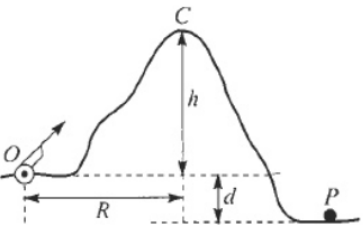
\includegraphics[width=0.7\linewidth]{screenshot003}
		\caption{Sistema de Polias.}
		\label{fig:fig3}
	\end{figure}

	\begin{parts}
		\part Desenhe o diagrama das forças que atuam em cada um dos corpos;

		\begin{solution}

		\end{solution}

		\part Como você pode escrever de forma matemática o vínculo entre os corpos devido às cordas?

		\begin{solution}

		\end{solution}

		\part Escreva as equações do movimento para cada um dos corpos?

		\begin{solution}

		\end{solution}

		\part A energia é conservada no sistema?

		\begin{solution}

		\end{solution}

		\part Considerando o sistema $ M_1 + M_2 + M_3 $, o momento linear é conservado? Por quê?

		\begin{solution}

		\end{solution}
	\end{parts}

	\medskip

	\question Um caminhão-tanque cheio de água, de massa total $ M $, utilizado para limpar ruas com um jato de água, trafega por uma via horizontal, com coeficiente de atrito cinético $\mu$. Ao atingir a velocidade $ v_0 $, o motorista coloca a marcha no ponto morto e liga o jato de água, que é enviada para trás com velocidade ve relativa ao caminhão, com uma vazão de $ \lambda $ litros por segundo. Ache a velocidade $ v(t) $ do caminhão depois de um tempo $ t $.

	\begin{solution}

	\end{solution}

\end{questions}
\end{document}
